\documentclass{article}
\usepackage{amsmath,amsfonts,amsthm,amssymb,amsopn,bm}
\usepackage[margin=.9in]{geometry}
\usepackage{graphicx}
\usepackage{url}
\usepackage[usenames,dvipsnames]{color}
\usepackage{fancyhdr}
\usepackage{multirow}
\usepackage{listings}
\usepackage{hyperref}

\definecolor{keywords}{RGB}{255,0,90}
\definecolor{comments}{RGB}{0,0,113}
\definecolor{red}{RGB}{160,0,0}
\definecolor{green}{RGB}{0,150,0}
 
\lstset{language=Python, 
        basicstyle=\ttfamily\tiny, 
        keywordstyle=\color{keywords},
        commentstyle=\color{comments},
        stringstyle=\color{red},
        showstringspaces=false}

\newcommand{\field}[1]{\mathbb{#1}}
\newcommand{\1}{\mathbf{1}}
\newcommand{\E}{\mathbb{E}} 
\newcommand{\Z}{\mathbb{Z}} 
\renewcommand{\P}{\mathbb{P}}
\newcommand{\R}{\field{R}} % real domain
% \newcommand{\C}{\field{C}} % complex domain
\newcommand{\F}{\field{F}} % functional domain
\newcommand{\T}{^{\textrm T}} % transpose
\def\diag{\text{diag}}

%% operator in linear algebra, functional analysis
\newcommand{\inner}[2]{#1\cdot #2}
\newcommand{\norm}[1]{\left\|#1\right\|}
\newcommand{\twonorm}[1]{\|#1\|_2^2}
% operator in functios, maps such as M: domain1 --> domain 2
\newcommand{\Map}[1]{\mathcal{#1}}
\renewcommand{\theenumi}{\alph{enumi}} 

\newcommand{\Perp}{\perp \! \! \! \perp}

\newcommand\independent{\protect\mathpalette{\protect\independenT}{\perp}}
\def\independenT#1#2{\mathrel{\rlap{$#1#2$}\mkern2mu{#1#2}}}
\newcommand{\vct}[1]{\boldsymbol{#1}} % vector
\newcommand{\mat}[1]{\boldsymbol{#1}} % matrix
\newcommand{\cst}[1]{\mathsf{#1}} % constant
\newcommand{\ProbOpr}[1]{\mathbb{#1}}
\newcommand{\points}[1]{\small\textcolor{magenta}{\emph{[#1 points]}} \normalsize}
\date{{}}

\setlength\parindent{0px}

\begin{document}
\title{Homework \#5}
\author{\normalsize{Winter 2020, STATS 509}\\
\normalsize{Dino Bektesevic}}
\maketitle



\section*{Problem 1}
Let $X_1$ and $X_2$ be independent random variables, with means $\mu_1$, $\mu_2$, and variances $\sigma^2_1$ and $\sigma^2_2$ respectively. Further, let $S = (X_1 + X_2)/2$ and $T = (X_1 - X_2)/2$. Find:
\begin{enumerate}
    \item[(a)] E$[S]$ and E$[T]$;

    \begin{align*}
        E[S] &= E[X_1/2 + X_2/2] \\
        &= \frac{1}{2}E[X_1] + \frac{1}{2}E[X_2] \\
        &= \frac{1}{2}\mu_1 + \frac{1}{2}\mu_2 \\
    \end{align*}
    
    \begin{align*}
        E[T] &= E[X_1/2 - X_2/2] \\
        &= \frac{1}{2}E[X_1] - \frac{1}{2}E[X_2] \\
        &= \frac{1}{2}\mu_1 - \frac{1}{2}\mu_2 \\
    \end{align*}
    
    \item[(b)] V$(S)$ and V$(T)$;

    \begin{align*}
        V[S] &= V[X_1/2 + X_2/2] \\
        &= \frac{1}{4}V[X_1] + \frac{1}{4}V[X_2] + \frac{1}{2}Cov(X_1, X_2)\\
        &= \frac{1}{4}\sigma_1 + \frac{1}{4}\sigma_2 \\
    \end{align*}
    
    \begin{align*}
        V[S] &= V[X_1/2 - X_2/2] \\
        &= \frac{1}{4}V[X_1] + \frac{1}{4}V[X_2] - \frac{1}{2}Cov(X_1, X_2)\\
        &= \frac{1}{4}\sigma_1 + \frac{1}{4}\sigma_2 \\
    \end{align*}

    \item[(c)] Cov$(S,T)$;

    \begin{align*}
        Cov(S, T) &= Cov\left(\frac{X_1}{2}+\frac{X_2}{2}, \frac{X_1}{2}-\frac{X_2}{2} \right) \\
        &= \frac{1}{4} Cov(X_1, X_1) - \frac{1}{4} Cov(X_1, X_2) - \frac{1}{4}Cov(X_2, X_1) + \frac{1}{4} Cov(X_2, X_1)\\
        &= \frac{\sigma_1}{4} + \frac{\sigma_2}{4} - \frac{1}{2}Cov(X_1, X_2) \\
        &= \frac{\sigma_1 + \sigma_2}{4}
    \end{align*}

    \item[(d)] Cov$(X_1,S)$, Cov$(X_2,T)$.
    
    $$Cov\left(X_1, \frac{X_1}{2}+\frac{X_2}{2}\right) = \frac{1}{2} Cov(X_1, X_1) =  \frac{\sigma_1}{2} $$
    $$Cov\left(X_2, \frac{X_1}{2}-\frac{X_2}{2}\right) = -\frac{1}{2} Cov(X_2, X_2) =  -\frac{\sigma_2}{2} $$
\end{enumerate}



\newpage
\section*{Problem 2}
Suppose that $X$ is a continuous random variable with support on $\mathbb{R}$. Suppose that the pdf for $X$ is symmetric around a point $t$, so that $f(t-x) = f(t+x)$ for all $x$.
\begin{enumerate}
    \item Find the median of $X$. {\it Hint: use the fact that the pdf integrates to $1$ and then split the integral into two pieces.}
    
    \begin{align*}
        1 &= \int_{-\infty}^\infty f_X dx \\
        &= \int_{-\infty}^t f(x)dx + \int_t^\infty f(x)dx \\
        &= 2\int_{-\infty}^t f(x)dx  \\
        &= 2F(X=t) \\
        &\rightarrow F(X=t) = \frac{1}{2}
    \end{align*}
    Since the median is defined as $F(X=t')=1/2$ this implies $t$ is the median of $X$.
    
    \item Find the mean of $X$. {\it Hint: use the fact that $E[X] = t^*$ if and only if $E[X-t^*]=0$. Again split the integral; also see Midterm Qu.3(b)} 
    
    \begin{align*}
        E[X-t] &= \int_{-\infty}^\infty (x-t) f(x) dx \\
        0 &= \int_{-\infty}^\infty x f(x) dx - t \int_{-\infty}^\infty f(x) dx \\
        0 &= E[X] - t \\
        E[X] &=  t
    \end{align*}
    
\end{enumerate}



\newpage
\section*{Problem 3}
Consider a continuous random variable with pdf $f_X(x)$ and CDF $F_X(x)$.
\begin{enumerate}
    \item Show that $\int_{-\infty}^t F_X(x) dx = \int_{-\infty}^t f(u) (t-u) du$.\par {\it Hint: recall HW3 Qu.3}
    
    \begin{align*}
        \int_{-\infty}^t F_X(x) dx &= \int_{-\infty}^t\int_{-\infty}^x f(u)dudx \\
        &= \int_{-\infty}^x\int_{u}^t f(u)dudx \\
        &= \int_{-\infty}^t f(u)(t-u) du
    \end{align*}

    \item Similarly show that $\int_{t}^\infty (1-F_X(x)) dx = \int_{t}^\infty f(u) (u-t) du$.
    
    \begin{align*}
        \int_{-\infty}^t 1-F_X(x) dx &= \int_t^\infty\int_x^\infty f(u)dudx \\
        &= \int_x^\infty \int_t^u f(u)dudx \\
        &= \int_t^\infty f(u)(u-t) du
    \end{align*}
\end{enumerate}
Define $h(t) \equiv E|X-t|$; the average absolute value of the prediction error, when using the constant $t$ as a prediction (for all units).
\begin{enumerate}
    \item[(c)] Show that $h(t) =  \int_{-\infty}^t F_X(x) dx + \int_t^\infty(1 - F_X(x))dx$.
    
    \begin{align*}
        h(t) &= E[|X-t|] \\
        &= \int_{-\infty}^\infty |x-t| f(x) dx \\
        &= \int_{-\infty}^t |x-t| f(x) dx + \int_t^\infty |x-t|f(x)dx \\
        &= \int_{-\infty}^t (t-x) f(x) dx + \int_t^\infty (x-t)f(x)dx \\
        &=  \int_{-\infty}^t F(x) dx + \int_t^\infty 1-F(x) dx 
    \end{align*}

    \newpage
    \item[(d)] Using your answer to (c) show that $h(t)$ is minimized when $t$ is a median for $X$. Recall that $m$ is a median for $X$ if $F_X(m) = 0.5$.\par
            {\it Hint: use the Fundamental Theorem of Calculus and your answer to (c).}
        
    \begin{align*}
        \frac{\partial}{\partial t}h(x) &= \frac{\partial}{\partial t}  \int_{-\infty}^t F(x) dx - \int_{-\infty}^t 1-F(x) dx  \\
        &= F(x) - 1 + F(x) 
    \end{align*}
    Minimizing $h(t)$:
    \begin{align*}
    h'(t) &= 0 \\
    2F(t) - 1 &= 0 \\
    F(t) = \frac{1}{2}
    \end{align*}
    and lets just assume the second derivative is positive, making this the minimum. 
    
\end{enumerate}



\newpage
\section*{Problem 4.} Goldberger Question 6.2
A known joint distribution of $X$ - price and $Y$ - quantity. Best linear predictor $E^*[X|Y]$ is used to predict quantity given price with an error $U = Y-E^*(Y|X)$. Other BLP predicts price given quantity with an error $V = X - E^*[X|Y]$. Let $\sigma_{XY} = C(X,Y)$ and $\sigma_{UV} = C(U,V)$ and $\rho$ the correlation of $X$ and $Y$. 

\begin{enumerate}
    \item Show $\sigma_{UV} = (1 - \rho^2)\sigma_{XY}$
        \begin{align*}
            \sigma_{UV} &= Cov(U,V) = Cov(Y - E[Y|X], X-E[X|Y]) \\
            &= Cov(X, Y) - Cov(Y, E[X|Y]) - Cov(X, E[Y|X]) + Cov(E[Y|X], E[X|Y]) \\
            &= Cov(X,Y) - Cov(Y, d+cY) = - Cov(X, b+aX) + Cov(d+cY b+aX) \\
        \end{align*}
    but since they used a linear predictor we know that 
        \begin{align*}
            a &= E[X] - bE[X] \\
            b &=  \frac{Cov(X,Y)}{V(X)} \\
            c &= \frac{Cov(X,Y)}{V(Y)} \\
            d &= E[Y] - cE[Y]
        \end{align*}
    substituting, canceling terms and using the definition of correlation $\rho = \frac{Cov(X,Y)}{\sigma_X\sigma_Y}$ then gives us:
        \begin{align*}
            \sigma_{UV} &= Cov(X,Y) - cV(Y) - aV(X) + bdCov(X,y) \\
            &= Cov(X,Y)(1+bd) - cV(Y) - aV(X) \\
            &= Cov(X,Y)(1+\rho^2) - 2Cov(X,Y) \\
            &= \rho^2 Cov(X,Y) - Cov(X, Y) \\
            &= (\rho^2-1) Cov(X, Y)
        \end{align*}
        
    \item Since $0 \leq \rho^2 \leq 1$ by Cauchy-Schwartz inequality, we can say that $-\sigma_{UV} \leq \sigma_{XY}$
\end{enumerate}


\newpage
\section*{Problem 5.} 

For this question use the following dataset:\par
{\scriptsize \url{http://www.stat.washington.edu/tsr/s509/examples/pres-election-2016-pop-density.csv}}\par
The dataset contains two variables measured in every US county:
\begin{enumerate}
    \item {\tt log10popdens}: the logarithm (base 10) of the population density measured in people per square kilometer;
    \item{\tt logpartyratio}: the natural logarithm of the ratio of the vote share for Hillary Clinton to the vote share for Donald Trump in 2016.
\end{enumerate}
The dataset also contains the county name and the state. Using {\tt R} or a similar package find:
\begin{enumerate}
    \item[(a)] The best linear predictor of {\tt logpartyratio} from  {\tt log10popdens}.
    \item[(b)] The approximate conditional expectation function\par
        E[ {\tt logpartyratio} $|$ {\tt log10popdens} ] by dividing {\tt log10popdens} into 13 bins:
        $$(-2.0,-1.5], (-1.5,-1.0], \ldots ,(4.0,4.5]$$
        and computing the mean in each bin.\par
        {\it Hint: In {\tt R} these are the bins given by the {\tt hist} function.}
    \item[(c)] The conditional expectation function via the loess smoother for\par
        E[ {\tt logpartyratio} $|$ {\tt log10popdens} ]
\end{enumerate}
Construct a scatterplot showing the data together with these three functions. Also provide the code that you used. {\it  See the example code here:}\url{http://www.stat.washington.edu/tsr/s509/examples/edwage.r}

\begin{center}
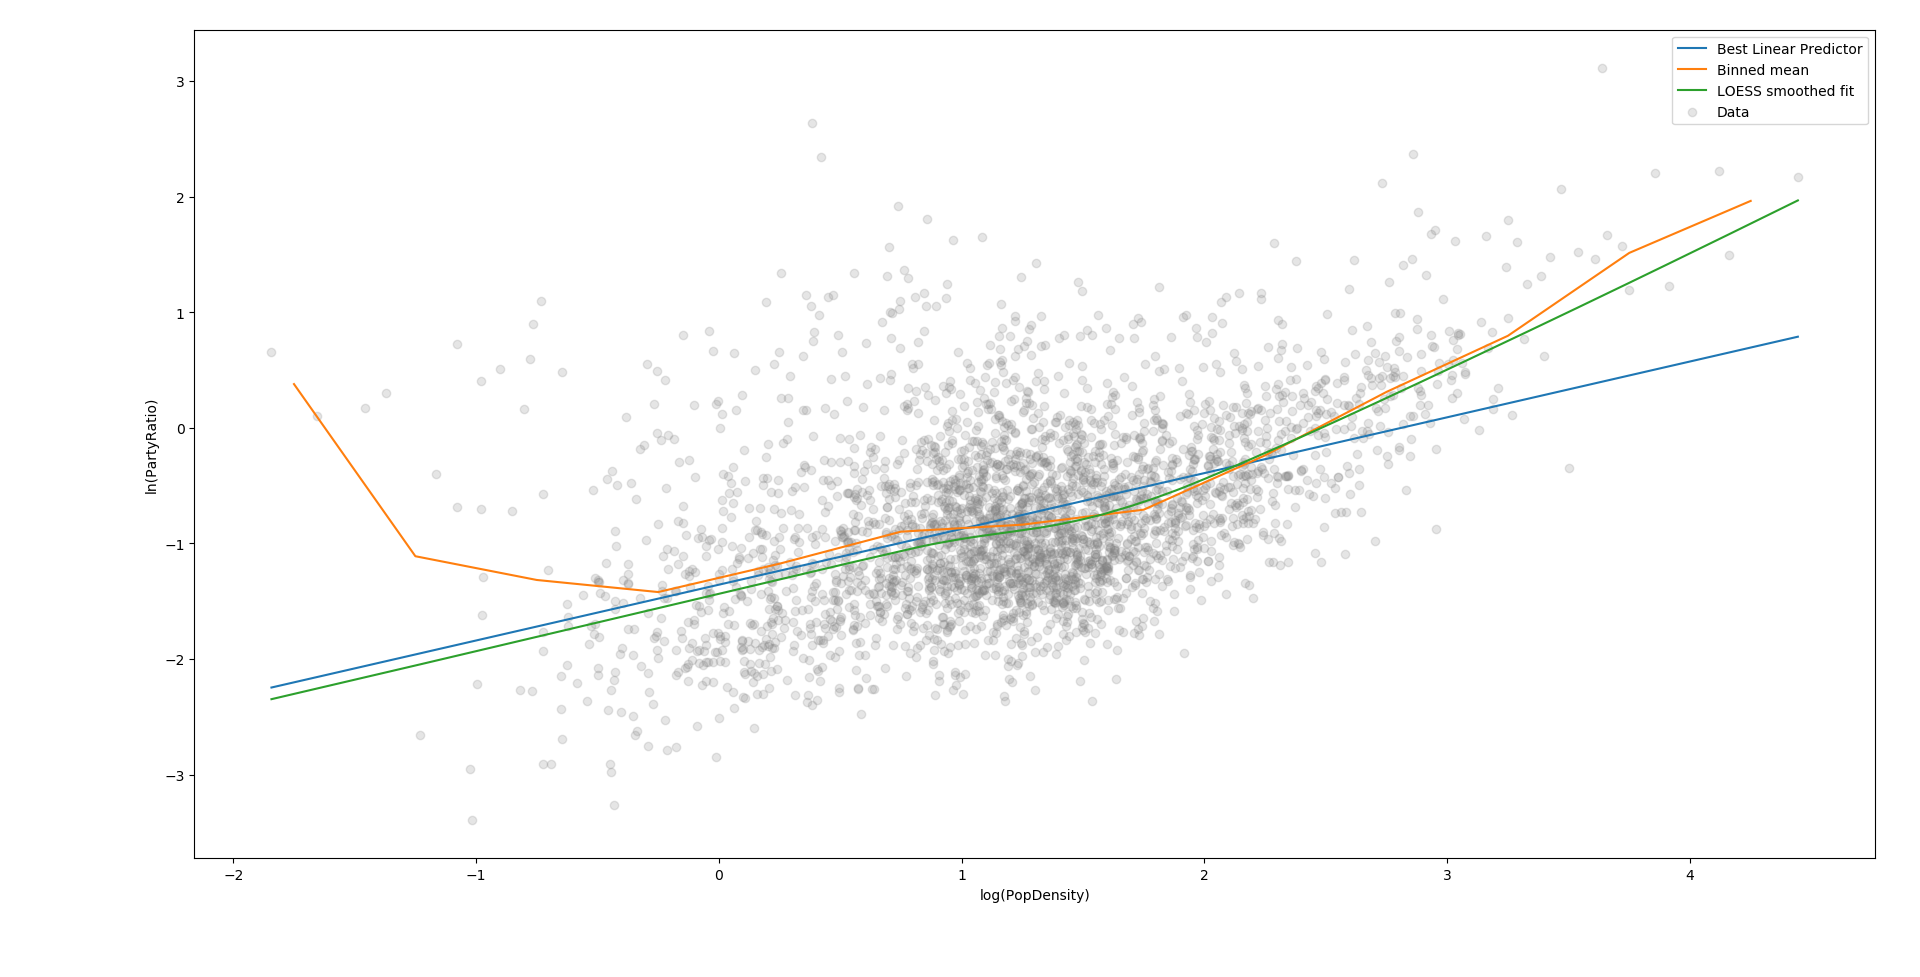
\includegraphics[width=500px]{STATS509/HW5/problem5.png}
\end{center}

\newpage
\lstinputlisting[language=Python]{HW5Code/HW5_DinoBektesevic.py}


\newpage
\section*{Problem 6.}
A population consists of two types, {\it humans} and {\it replicants}. The proportion of replicants is $q$. The height of each type approximately follow normal distributions. Let $N(\mu_H,\sigma^2_H)$ be the distribution of lengths for humans; let $N(\mu_R,\sigma^2_R)$ be the distribution of lengths for replicants.
\begin{enumerate}
    \item Find the mean height of a randomly sampled subject in this population.
    
    $$E(X) = E_T[E(X|T)] = E_T(\mu_{X|T}) = q\mu_R + (1-q)\mu_H$$
    
    \item Find the variance of the distribution of height for subjects in this population.
    
    \begin{align*}
        V(X) &= E_T[V[X|T]) + V(E[X|T]) = E(\sigma_{Y|X}^2) + V(\mu_{Y|X}) \\
        &= q\sigma_R^2 + (1-q)\sigma_H^2 + E[\mu_{Y|X}] - E[\mu_{Y|X}]^2 \\
        &= q\sigma_R^2 + (1-q)\sigma_H^2 + (1-q)\mu_H^2 + q\mu_R^2 - \left[ (1-q)\mu_H + q\mu_R \right]^2\\
        &= q\sigma_R^2 + (1-q)\sigma_H^2 + (1-q)\mu_H^2 + q\mu_R^2 - \left[ (1-q)^2\mu_H^2 + 2q(1-q)\mu_H\mu_R + q^2\mu_R^2 \right]\\
        &= q\sigma_R^2 + (1-q)\sigma_H^2 + (1-q)\left[\mu_H^2 - (1-q)\mu_H^2 - 2q\mu_H\mu_R \right] \\
        &= q\sigma_R^2 + (1-q)\sigma_H^2 + (1-q)\left[q\mu_H^2 - 2q\mu_H\mu_R \right] \\
        &= q\sigma_R^2 + (1-q)\sigma_H^2 + q(1-q)(\mu_H - 2\mu_R)\mu_H
    \end{align*}
\end{enumerate}



\newpage
\section*{Problem 7}
Suppose that $X$ and $Y$ are continuous random variables, with support on $\mathbb{R}^2$.
Suppose that two researchers, Thelma and Louise, wish to predict $Y$ from $X$ using a function of $X$.
\begin{enumerate}
    \item Thelma wishes to use the function $g_T(X)$ that minimizes  the average squared prediction $E[(Y-g_T(X))^2]$. What function will Thelma use? {\it You may justify your answer by quoting results from the Lecture.}
    
    Golberger chapter 5.4:
    $$g_T(X) = E[Y|X]$$
    
    \item Louise, however, wishes to use the function $g_L(X)$ that minimizes the average absolute error $E[|Y-g_L(X)|]$. What function will Louise choose?  Explain your answer. {\it Hint: Use the law of iterated expectations and Qu.3.}
    
    We find a functional expression for $E[|Y-g_L(X)|]$ and then minimize it:
    \begin{align*}
    \min E[|Y-g_L(X)|] &= \min E\left[E\left[|Y-g_L(X)|| X \right] \right] \\
    &= \min \int_{-\infty}^{\infty}\left(\int_{-\infty}^\infty |y-g_L(x)|f_{Y|X}(y|x)dy\right) f_{X}(x)dx \\
    &= \int_{-\infty}^{\infty} \min \left(\int_{-\infty}^\infty |y-g_L(x)|f_{Y|X}(y|x)dy\right)f_{X}(x)dx  \\
    \end{align*}
    Minimizing the inside integral is essentially problem 3, because when $X=x \rightarrow g_L(X)=c$ and goes as:
    \begin{align*}
    \min E\left[|Y-g_L(X)|| X \right]  &= \min\left( \int_{-\infty}^{g_L(X)} (g_L(X) - y) f_{Y|X}(y|x) dy  + \int_{g_L(X)}^\infty (y-g_L(X)) f_{Y|X}(y|x) dy \right)\\
    0 &= \frac{\partial}{\partial g_L(X)} \left[  \int_{-\infty}^{g_L(X)} (g_L(X) - y) f_{Y|X}(y) dy  + \int_{g_L(X)}^\infty (y-g_L(X)) f_{Y|X}(y) dy  \right] \\
    0 &= \int_{-\infty}^{g_L(X)} f_{Y|X}(y) dy  - \int_{g_L(X)}^\infty f_{Y|X}(y) dy  \\
    0 &= F_{Y|X}\left[ g_L(X)\right]  - 1 + F_{Y|X}\left[g_L(X)\right] \\
    0 &= 2 F_{Y|X}\left[g_L(X)\right] - 1 \\
    F\left[g_L(X)\right] &= \frac{1}{2}
    \end{align*}
    Implying $\min E[|Y-g_L(X)|]$ will coincide with the median. 
    
    \newpage
    I spent a lot of time conversing with professor Thomas about why that minimum function can be moved into the integral and why is the minimum of the internal integral also the minimum of the internal integral times f. As per his instructions there is an alternative way that avoids explicitly explaining those points. The same can be proven then as follows. Let $g_L(x)$ be some function and let 
    
    \begin{align*}
        h_1(x) &= E[|Y-med(Y|X)| | X=x] \\
        h_2(x) &= E[|Y-g(X)|| X=x]
    \end{align*}
    By question 3 we have that for all x:
    \begin{align*}
    h_1(x) &\leq h_2(x) \\ 
    E[|Y-med(Y|X)|| X=x]  &\leq E[|Y-g(X)|| X=x]
    \end{align*}
    Consequently $h(x) - h^*(x) \geq 0$ for all $x$. That motivates defining
    $$q(x) = h^*(x) -h(x)$$
    So that 
    $$ E[G_L(X)] = \int_{-\infty}^{\infty} q(x)f_X(x)dx $$
    We know that $q(x) \geq 0$ for all $x$ as shown above. Hence $E[q(X)] \geq 0$. Therefore 
    $$\int_{-\infty}^{\infty} q(x)f_X(x)dx \geq 0.$$
    we have the integral we started off with in my solution writeup. But then instead of struggling with moving the minimization into the integral explanation we can instead by definition of $q$ write:
    $$E_{X} [E[|Y-g(X)||X] - E[|Y-med(Y|X)||X] ] \geq 0 $$ 
    where expectation of sum is sum of expectations:
    $$E_{X}[E[|Y-g(X)||X]] - E_{X} [E[|Y-med(Y|X)||X]] \geq 0 $$   
    and applying law of iterated expectations in reverse:
    \begin{align*}
    E[|Y-g(X)|] - E[|Y-med(Y|X)|]  &\geq 0 \\
    E[|Y-g(X)|] \geq E[|Y-med(Y|X)|]
    \end{align*}
    Implying that the median is the optimal minimizer of the problem and that Louise should use the median, which is the same conclusion we reach above.
    
    \item Suppose that there is a function $r(x)$ such that the conditional density for $Y$ given $X=x$ is symmetric around $r(x)$, so that for all $x$ and $y$, $f(r(x) - y \,|\,x) =  f(r(x)+y \,|\,x)$, what can we say about the functions $g_T(X)$ and $g_L(X)$ used by Thelma and Louise? {\it Hint: Use Qu.2.}
    
    They would be equal because from Qu. 2. we know that $E[Y|X]=r(x)$ when distribution is symmetric around $r(x)$ and we also know that if the conditional density is symmetric around $r(x)$ then $r(x)$ will be the median of the conditional density. 
    
\end{enumerate}



\newpage
\section*{Problem 8} Suppose a medical test has the following characteristics:
\begin{eqnarray*}
    Pr(\hbox{Test +ve} \mid \hbox{Patient Diseased})&=& 0.99\\
    Pr(\hbox{Test -ve} \mid \hbox{Patient Not Diseased})&=& 0.98
\end{eqnarray*}

\begin{enumerate}
    \item[(a)] Find $Pr(\hbox{Test -ve} \mid $ Patient Diseased $)$ and $Pr(\hbox{Test +ve} \mid$ Patient Not Diseased $)$.
    
    $$P(-|sick) = 1 - P(+|healthy) = 0.01$$
    $$P(+|healthy) = 1 - P(-|sick) = 0.02$$
    
\end{enumerate}

Suppose that 1 in 5,000 people have this disease so $Pr(\hbox{Patient Diseased}) = 0.0002$
\begin{enumerate}
    \item[(b)] Compute $Pr( \hbox{Test +ve} )$. {\it Hint: Find $Pr(\hbox{Test +ve},$ {Patient Diseased}$)$ and $Pr(\hbox{Test +ve},$ {Patient Not Diseased}$)$.}
    
    \begin{align*}
        P(+) &= P(+|healthy) P(healthy) + P(+|sick)P(sick) \\
        &= 0.02\cdot (1-0.0002) + 0.99\cdot 0.0002 \\
        &= 0.02
    \end{align*}
    
    \item[(c)] Use Bayes' rule to find $Pr(\hbox{Patient Diseased} | {Test +ve})$.
    
    $$P(sick|+) = \frac{P(+|sick)P(sick)}{P(+)} = \frac{0.99\cdot 0.0002}{0.02} \approx 0.01$$

    \item[(d)] Give an intuitive explanation for the discrepancy between $Pr($ Patient Diseased $|$ {Test +ve}$)$ and $Pr($ {Test +ve} $|$ Patient Diseased).
    
    When the number of tested people is very large, the number of false positives will be very large even when the false positive rate is small (2\% in this example). At the same time the number of people that are sick is relatively small, thus the number of true positives will be small as well. Therefore $P(+|sick)$ can be very large but $P(sick|+)$ can still be rather small. 
    
    
\end{enumerate}
\end{document}
